\chapter{Eigenvalues of Infinite Matrices}
This chapter centers its attention on eigenvalues and eigenvectors within the context of infinite matrices. Section 1 serves as a comprehensive introduction to these fundamental concepts, particularly emphasizing methodologies, practical applications, and their significance in the realm of finite matrices. The subsequent transition to Section 2 involves an in-depth analysis of eigenvalues and eigenvectors within the domain of infinite matrices. This analytical exploration encompasses the resolution of characteristic equations, employing determinant and identity matrices, and addresses computational intricacies, such as exponentiation and logarithmic transformations. The systematic elucidation of each eigenvalue and its corresponding eigenvector contribute valuable insights into the inherent properties characterizing infinite matrices.



\section{Eigenvalues of a finite matrix}
\label{sec:intro_eigen}


Let $A$ be a square matrix of order $n$ and ${X} \in \mathbb{C}^n $ be a nonzero vector for which
\begin{center}
    $A{X} = \lambda {X} $
\end{center}
for some scalar $ \lambda \in \mathbb{C}$. Then $ \lambda $ is called an \textbf{eigenvalue} of the matrix $ A $, and $ {X} $ is called an \textbf{eigenvector} of $ A $ associated to $ \lambda $. The set of all eigenvalues of a matrix $ A $ is denoted by $ \sigma(A) $ and is referred to as the spectrum of $ A $.    


\begin{example}
    Find the eigenvalues of the matrix \[ A = \begin{bmatrix} 2 & 2 \\ 5 & -1 \end{bmatrix}. \]

The eigenvalues are those \( \lambda \) for which \( \text{det}(A - \lambda I) = 0 \). Now 
$$
\begin{aligned}
\operatorname{det}({A}-\lambda {I}) & =\operatorname{det}\left(\left[\begin{array}{cc}
2 & 2 \\
5 & -1
\end{array}\right]-\lambda\left[\begin{array}{ll}
1 & 0 \\
0 & 1
\end{array}\right]\right) \\
& =\operatorname{det}\left(\left[\begin{array}{cc}
2 & 2 \\
5 & -1
\end{array}\right]-\left[\begin{array}{cc}
\lambda & 0 \\
0 & \lambda
\end{array}\right]\right) \\
& =\left|\begin{array}{cc}
2-\lambda & 2 \\
5 & -1-\lambda
\end{array}\right| \\
& =(2-\lambda)(-1-\lambda)-10 \\
& =\lambda^2-\lambda-12 .
\end{aligned}
$$



The eigenvalues of \( A \) are the solutions of the quadratic equation \( \lambda^2 - \lambda - 12 = 0 \), namely \( \lambda_1 = -3 \) and \( \lambda_2 = 4 \).

As we have discussed, if \( \text{det}(A - \lambda I) = 0 \), then the equation \( (A - \lambda I)x = b \) has either no solutions or infinitely many. When we take \( b = 0 \), however, it is clear by the existence of the solution \( x = 0 \) that there are infinitely many solutions (i.e., we may rule out the "no solution" case). If we continue using the matrix \( A \) from the example above, we can expect nonzero solutions \( x \) (infinitely many of them, in fact) of the equation \( Ax = \lambda x \) precisely when \( \lambda = -3 \) or \( \lambda = 4 \). Let us proceed to characterize such solutions.

First, we work with \( \lambda = -3 \). The equation \( Ax = \lambda x \) becomes \( Ax = -3x \). Writing \( x = \begin{bmatrix} x_1 \\ x_2 \end{bmatrix} \) and using the matrix \( A \) from above, we have 
\[
\begin{aligned}
    Ax &= \begin{bmatrix} 2x_1 + 2x_2 \\ 5x_1 - x_2 \end{bmatrix}, \\
    -3x &= \begin{bmatrix} -3x_1 \\ -3x_2 \end{bmatrix}.
\end{aligned}
\]
Setting these equal, we get
$$
\begin{aligned}
{\left[\begin{array}{c}
2 x_1+2 x_2 \\
5 x_1-x_2
\end{array}\right]=\left[\begin{array}{c}
-3 x_1 \\
-3 x_2
\end{array}\right] } & \Rightarrow 2 x_1+2 x_2=-3 x_1 \quad \text { and } \quad 5 x_1-x_2=-3 x_2 \\
& \Rightarrow 5 x_1=-2 x_2 \\
& \Rightarrow x_1=-\frac{2}{5} x_2 .
\end{aligned}
$$

This means that, while there are infinitely many nonzero solutions (solution vectors) of the equation ${A x}=-3 {x}$, they all satisfy the condition that the first entry $x_1$ is $-2 / 5$ times the second entry $x_2$. Thus all solutions of this equation can be characterized by
$$
\left[\begin{array}{c}
2 t \\
-5 t
\end{array}\right]=t\left[\begin{array}{c}
2 \\
-5
\end{array}\right],
$$

 where \( t \) is any real number. The nonzero vectors \( x \) that satisfy \( Ax = -3x \) are called eigenvectors associated with the eigenvalue \( \lambda = -3 \). One such eigenvector is \( u_1 = \begin{bmatrix} 2 \\ -5 \end{bmatrix} \), and all other eigenvectors corresponding to the eigenvalue \((-3)\) are simply scalar multiples of \( u_1 \) i.e. \( u_1 \) spans this set of eigenvectors.

Similarly, we can find eigenvectors associated with the eigenvalue \( \lambda = 4 \) by solving \( Ax = 4x \) as follows:
\[
\begin{aligned}
    \begin{bmatrix} 2x_1 + 2x_2 \\ 5x_1 - x_2 \end{bmatrix} &= \begin{bmatrix} 4x_1 \\ 4x_2 \end{bmatrix} 
\end{aligned}
\]
\[
\begin{aligned}
    &\Rightarrow 2x_1 + 2x_2 = 4x_1 \text{ and } 5x_1 - x_2 = 4x_2 \\
    &\Rightarrow x_1 = x_2
\end{aligned}
\]

Hence, the set of eigenvectors associated with \( \lambda = 4 \) is spanned by \( u_2 = \begin{bmatrix} 1 \\ 1 \end{bmatrix} \).
\end{example}



%\subsection{Should we add?}
%For a real matrix, the logarithm exists if and only if all its eigenvalues are positive. Specifically, the logarithm of a real matrix $A$ exists if and only if $A$ is positive definite, meaning that all its eigenvalues are strictly positive.\newline
%
%In the provided MATLAB \ref{lst:matrices-real-number} code, the attempt to generate a matrix with positive real eigenvalues is essential to ensure that the logarithm calculation using the series expansion is meaningful and converges to a valid result.
%
%Generated matrix with positive real eigenvalues and norm($I$ - $A$) $< 1$ after $261$ attempts.
%
%Original Matrix $A$:
%\[ A =
%    \begin{bmatrix}
%        1.3072 & 0.3070 & -0.4733 \\
%        -0.0204 & 0.3143 & 0.3128 \\
%        -0.5614 & 0.1224 & 0.9682
%    \end{bmatrix}
%\]
%
%Eigenvalues of $A$:
%\[
%    \begin{bmatrix}
%        1.6492 \\
%        0.7691 \\
%        0.1715
%    \end{bmatrix}
%\]
%
%Norm of $(I-A)$: 0.929513
%
%Original matrix determinant (up to 10 decimal places): 0.2175165714
%
%Approximated determinant after 98 iterations: 0.2175165715
%
%Final Determinant Error: 0.0000000001
%
%\[
%    \begin{bmatrix}
%        0.1199 & 0.6028 & -0.5924 \\
%        0.1597 & -1.3680 & 0.6558 \\
%        -0.5730 & 0.4526 & -0.2773
%    \end{bmatrix}
%\]\newline
% A complex matrix has a logarithm if and only if it is invertible. The logarithm is not unique, but if a matrix has no negative real eigenvalues, then there is a unique logarithm that has eigenvalues all lying in the strip $\{z \in \mathbb{C} \ \vert \ -\pi < \textit{Im} \ z < \pi\}$. This logarithm is known as the principal logarithm.
%
%The answer is more involved in the real setting. A real matrix has a real logarithm if and only if it is invertible and each Jordan block belonging to a negative eigenvalue occurs an even number of times. If an invertible real matrix does not satisfy the condition with the Jordan blocks, then it has only non-real logarithms. This can already be seen in the scalar case: no branch of the logarithm can be real at -1. The existence of real matrix logarithms of real $2 \times 2$ matrices is considered in a later section.
%
%
%
%
%Generated complex matrix with eigenvalues in the strip and norm less than $1$ after $401$ attempts.
%
%Original Complex Matrix $A$:
%\[
%\begin{bmatrix}
%   0.3145 - 0.6665i & -0.1452 - 0.1428i \\
%   0.0042 - 0.0410i & 1.0970 + 0.4197i
%\end{bmatrix}
%\]
%
%Eigenvalues of $A$:
%\[
%\begin{bmatrix}
%   0.3140 - 0.6727i \\
%   1.0975 + 0.4259i
%\end{bmatrix}
%\]
%
%Original matrix determinant:
%\[
%0.6311 - 0.6045i
%\]
%
%Approximated Logarithm of $A$ using series expansion:
%\[
%\begin{bmatrix}
%  -0.2998 - 1.1272i & -0.1079 - 0.2115i \\
%   0.0198 - 0.0439i & 0.1650 + 0.3631i
%\end{bmatrix}
%\]
%
%$\text{exp(trace}(\text{Log}A))$:
%\[
%0.6309 - 0.6046i
%\]
%\begin{center}
%   \begin{figure}
%    \centering
%    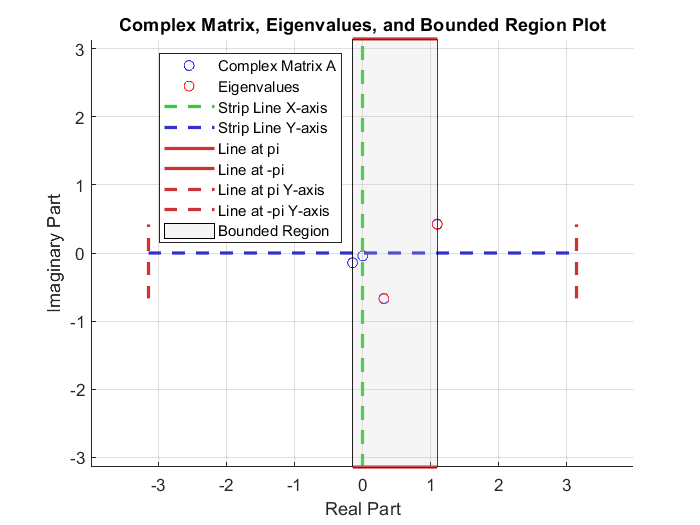
\includegraphics[width=0.8\linewidth]{Figures/eeeeeeeeeeeeeeeeeee.png}
%    \caption{logarithm of complex matrix}
%    \label{fig:complex}
%    \end{figure} 
%\end{center}
%
%This graph\ref{fig:complex} shows the complex matrix elements, eigenvalues, and bounded region plot. It is a way of visualizing the properties of complex matrices and their eigenvalues. The eigenvalues are the blue crosses on the graph, and they are the solutions of the characteristic equation of the matrix. The unit circle is the blue dashed circle, and it is the set of complex numbers with magnitude one. The bounded region is the shaded area, and it is the region where the matrix norm is less than one. The strips and lines are related to the convergence and divergence of the matrix power series. This graph is part of an application that allows you to explore infinite matrices and their results.
%



\bigskip
\section{Eigenvalues of an infinite matrix }

Let $A$ be any infinite square matrix. The $\operatorname{tr}(\log(A - \lambda I))$, where $\lambda$ is a scalar, is a logarithmic series. We note that $\operatorname{tr}(\log(A - \lambda I)) = \sum_{k=1}^{\infty} (-1)^{k+1}\operatorname{tr}(\frac{(A-\lambda I-I)^k}{k})$. 

\begin{definition}\label{eigenvalues_of_an_infinite_matrix}
Let $A$ be an infinite square matrix such that $\operatorname{tr}(\log(A - \lambda I))$ is a convergent series for some scalars $\lambda$. Then $\lambda$ is called an \textbf{eigenvalue} of the infinite matrix $A$ if and only if $$\exp(\operatorname{tr}(\log(A - \lambda I)))=0.$$
\end{definition}

We see that the above definition agrees the definition of the eigenvalues of a finite matrix $A$. Because, if $\lambda$ is an eigenvalue of $A$, by using the definition of the determinant of an infinite square matrix, we have 
\[
\text{det}(A - \lambda I) = \exp(\operatorname{tr}(\log(A - \lambda I))) = 0.
\]


As in the definition of the eigenvalues of an infinite square matrix, to find all the eigenvalues of an infinite matrix $A$, we must solve the equation $\exp(\operatorname{tr}(\log(A - \lambda I)))=0$ for all possible values of $\lambda$. In the following example, we use this definition in the case of the eigenvalues of a finite matrix. Here, we use the MATLAB code Source Code~\ref{sourcecode-eigenvalues} (Algorithm~\ref{alg-eig}). 


\begin{example}
% Generated matrix with positive real eigenvalues and norm(identity - A) < 1 after 9 attempts.


Let
\[A = 
\begin{bmatrix}
1.2000 & -0.0200 & -0.1200 & -0.0600 & -0.0800 & -0.0030 & -0.0050 \\
-0.0800 & 0.9997 & -0.0030 & -0.0400 & -0.0200 & -0.0070 & -0.0060 \\
-0.0100 & -0.0100 & 0.9997 & -0.0060 & -0.0070 & -0.0040 & -0.0006 \\
-0.0300 & -0.0100 & -0.0200 & 0.9994 & -0.0200 & -0.0500 & -0.0700 \\
-0.0300 & -0.2141 & -0.0007 & -0.0942 & 0.9999 & -0.0009 & -0.0001 \\
-0.0800 & -0.0120 & -0.0004 & -0.0009 & -0.9890 & 0.9994 & -0.0005 \\
-0.0300 & -0.0010 & -0.0050 & -0.0020 & 0 & -0.3000 & 0.9998 \\
\end{bmatrix}.
\]

We find that $\|I-A\| = 0.995135$ which is less than 1. This ensures that we can compute the eigenvalues of $A$. We find the eigenvalues of $A$ as follows: 
 $$ \lambda_1 = 0.705572, \quad \lambda_2 = 1.007391, $$
 $$ \lambda_3 = 1.007391, \quad \lambda_4 = 1.200285, $$
 $$ \lambda_5 = 1.139452, \quad \lambda_6 = 1.139452, \text{ and }$$
 $$ \lambda_7 = 0.998357.$$

% Norm of (I-A): 0.606617
For $ \lambda_1 = 0.705572 $, we have 
   $$\det(A - \lambda_1 I)= 0.$$

Then $$\exp(\operatorname{trace}(\log (A -\lambda_1 I ))) = 0.000002.$$

Thus, the final determinant error for eigenvalue $\lambda_1 = 0.0000021186$ after $1000$ iterations.

%%%% 2 
For $\lambda_2 = 1.007391$, we have $$\det(A - \lambda_2 I)= 0.$$

Then
$$\exp(\operatorname{trace}(\log (A -\lambda_2 I )))= 0.000000.$$ 

Thus, the final determinant error for eigenvalue $\lambda_2 = 0.0000000000$ after $32$ iterations.

%%%%%% 3 
For $ \lambda_3 = 1.007391 $, we have 
   $$\det(A - \lambda_3 I)= 0.$$

Then $$\exp(\operatorname{trace}(\log (A -\lambda_3 I ))) = 0.000000.$$

Thus, the final determinant error for eigenvalue $\lambda_3 = 0.0000021186$ after $32$ iterations.

%% 4 
For $\lambda_4 = 1.200285$, we have $$\det(A - \lambda_4 I)= 0.$$

Then
$$\exp(\operatorname{trace}(\log (A -\lambda_4 I )))= 0.000000.$$ 

Thus, the final determinant error for eigenvalue $\lambda_4 = 0.0000000000$ after $5$ iterations.
%%%%% 5

For $\lambda_5 = 1.139452 $, we have 
   $$\det(A - \lambda_1 I)= 0.$$

Then $$\exp(\operatorname{trace}(\log (A -\lambda_5 I ))) = 0.00000.$$

Thus, the final determinant error for eigenvalue $\lambda_5 = 0.0000000001$ after $6$ iterations.

%%%% 6 
For $\lambda_6 = 1.139452 $, we have $$\det(A - \lambda_6 I)= 0.$$

Then
$$\exp(\operatorname{trace}(\log (A -\lambda_6 I )))= 0.000000.$$ 

Thus, the final determinant error for eigenvalue $\lambda_6 = 0.0000000001$ after $6$ iterations.

%%%%%% 7 
For $\lambda_7 = 0.998357 $, we have $$\det(A - \lambda_7 I)= 0.$$

Then
$$\exp(\operatorname{trace}(\log (A -\lambda_7 I )))= 0.0000000000.$$ 

Thus, the final determinant error for eigenvalue $\lambda_7 = 0.0000000000$ after $12$ iterations.



The graphical representations in Figure~\ref{fig-eigenvalue1} to Figure~\ref{fig-eigenvalue7} capture the convergence behavior of determinant errors associated with $7$ eigenvalues across a series of iterative steps.  This graph provides valuable insights into the iterative refinement process, illustrating how the determinant error diminishes over successive iterations, thus indicating the improving accuracy and convergence of the eigenvalue computations for the given matrix.

\begin{figure}[h]
    \centering
    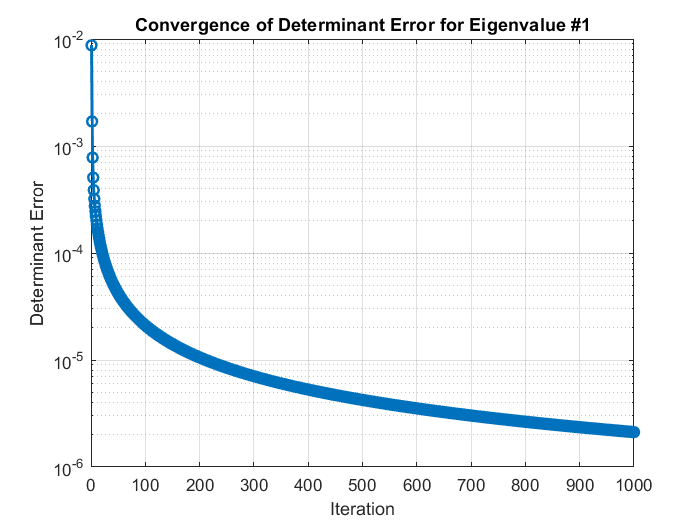
\includegraphics[width=.79\linewidth]{Figures/eigen_1.png}
    \caption{Error analysis of determinant for eigenvalue 1 }
    \label{fig-eigenvalue1}
\end{figure}

\begin{figure}[h]
    \centering
    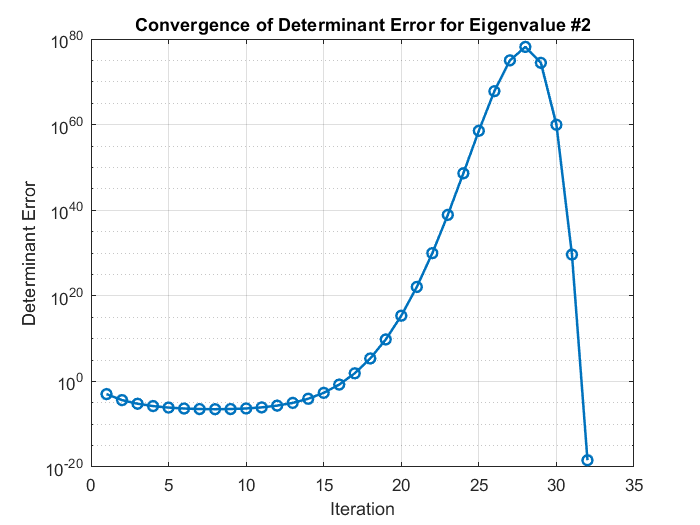
\includegraphics[width=.79\linewidth]{Figures/eigen_2.png}
    \caption{Error analysis of determinant for eigenvalue 2}
    \label{fig-eigenvalue2}
\end{figure}

\begin{figure}[h]
    \centering
    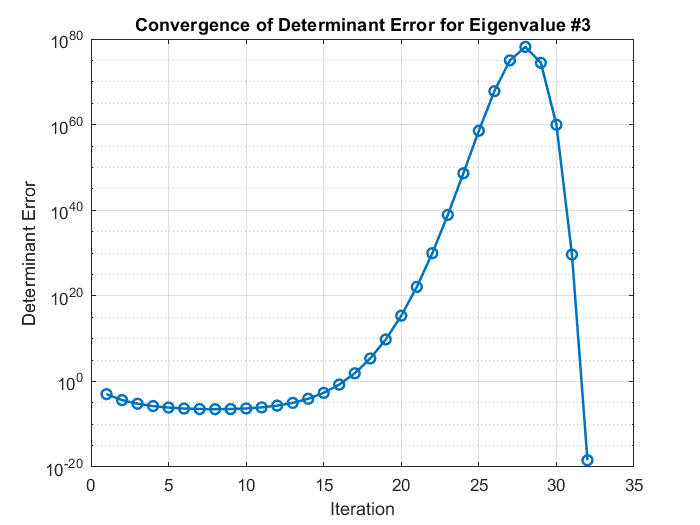
\includegraphics[width=.79\linewidth]{Figures/eigen_3.png}
    \caption{Error analysis of determinant for eigenvalue 3}
    \label{fig-eigenvalue3}
\end{figure}

\begin{figure}[h]
    \centering
    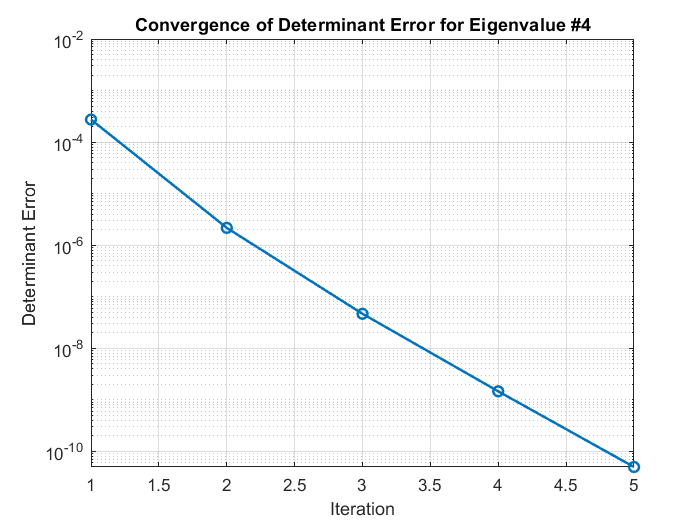
\includegraphics[width=.79\linewidth]{Figures/eigen_4.png}
    \caption{Error analysis of determinant for eigenvalue 4}
    \label{fig-eigenvalue4}
\end{figure}

\vspace{40pt}
\begin{figure}[h]
    \centering
    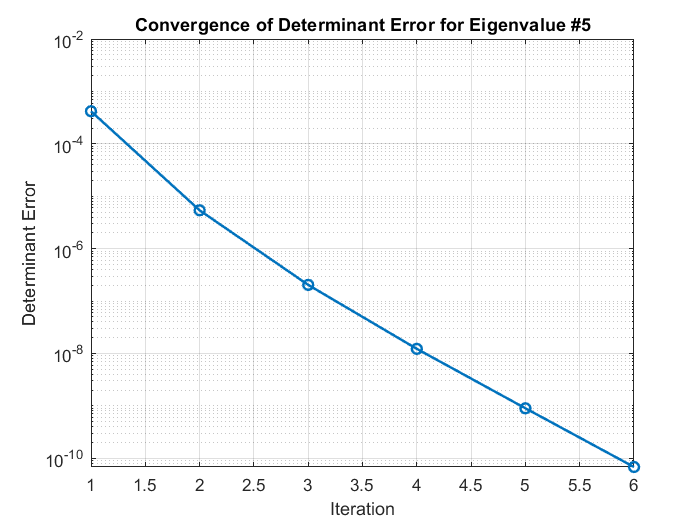
\includegraphics[width=.79\linewidth]{Figures/eigen_5.png}
    \caption{Error analysis of determinant for eigenvalue 5}
    \label{fig-eigenvalue5}
\end{figure}

\begin{figure}[h]
    \centering
    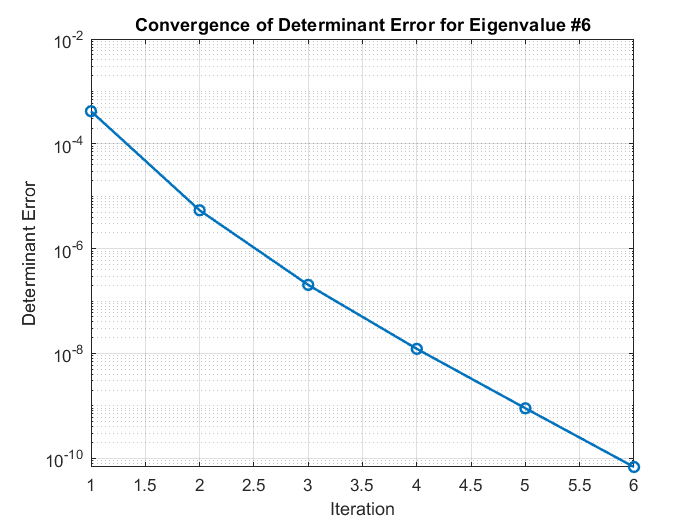
\includegraphics[width=.79\linewidth]{Figures/eigen_6.png}
    \caption{Error analysis of determinant for eigenvalue 6}
    \label{fig-eigenvalue6}
\end{figure}

\begin{figure}[h]
    \centering
    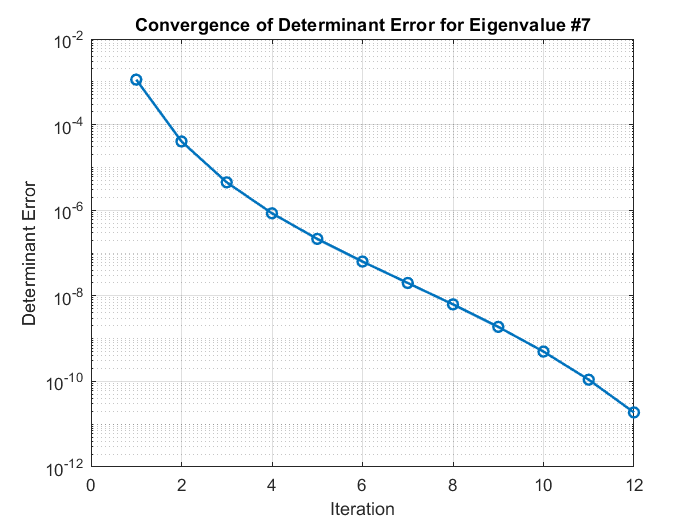
\includegraphics[width=.79\linewidth]{Figures/eigen_7..png}
    \caption{Error analysis of determinant for eigenvalue 7}
    \label{fig-eigenvalue7}
\end{figure}


% \begin{figure}[h]
%     \centering
% {0.3\linewidth}
%         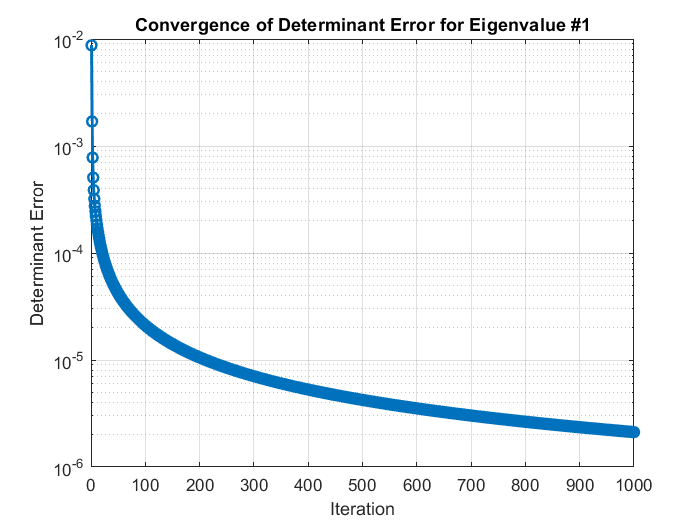
\includegraphics[width=\linewidth]{Figures/eigen_1.png}
%         \caption{Error Analysis 1}

%     \hfill
% {0.3\linewidth}
%         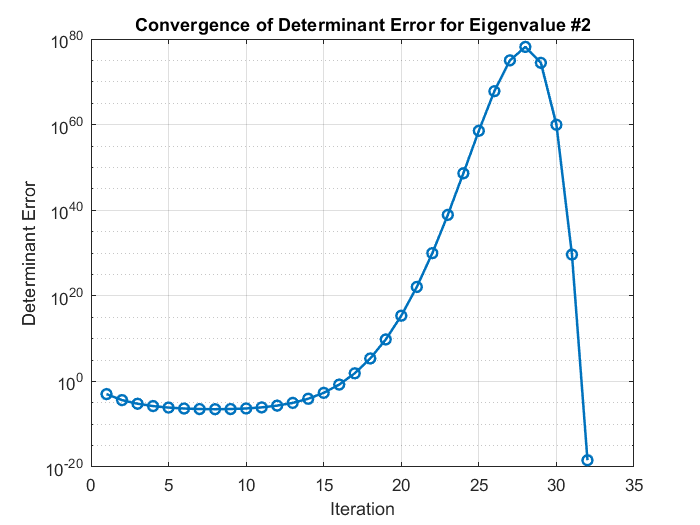
\includegraphics[width=\linewidth]{Figures/eigen_2.png}
%         \caption{Error Analysis 2}

%     \hfill
% {0.3\linewidth}
%         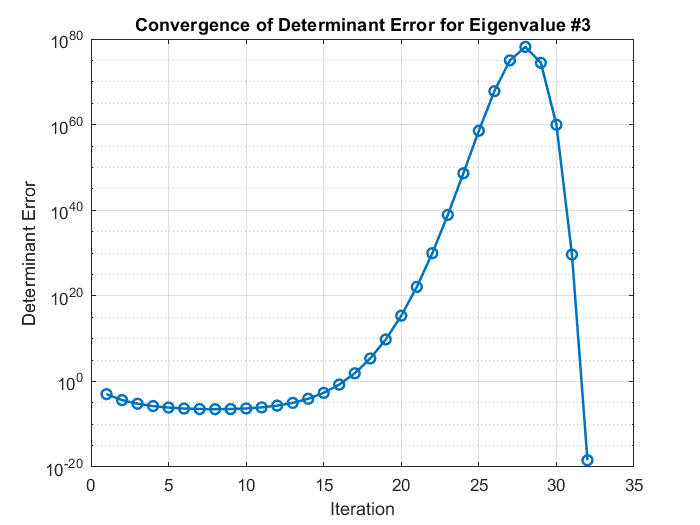
\includegraphics[width=\linewidth]{Figures/eigen_3.png}
%         \caption{Error Analysis 3}

    
%     \vspace{1em} % Add vertical space between rows
    
%     \begin{subfigure}{0.3\linewidth}
%         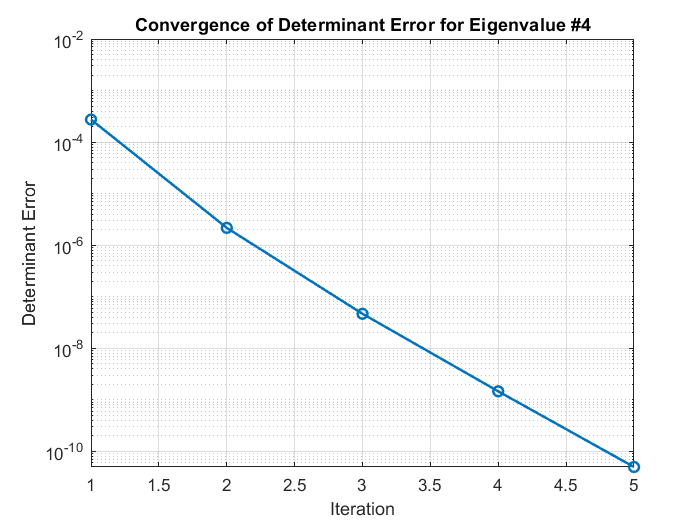
\includegraphics[width=\linewidth]{Figures/eigen_4.png}
%         \caption{Error Analysis 4}
%     \end{subfigure}
%     \hfill
%     \begin{subfigure}{0.3\linewidth}
%         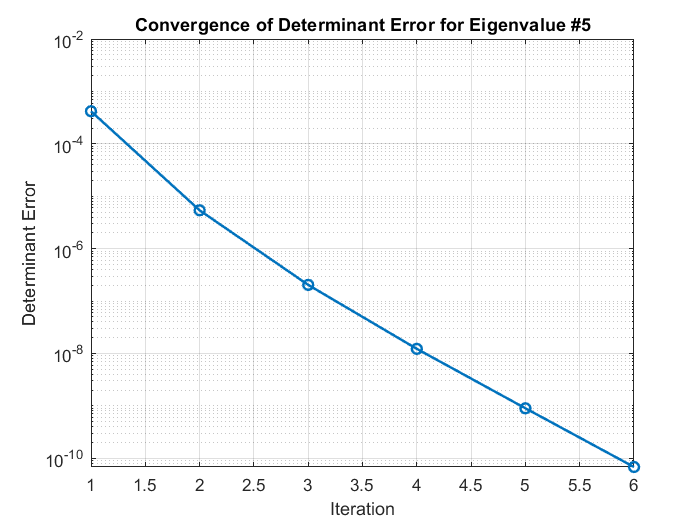
\includegraphics[width=\linewidth]{Figures/eigen_5.png}
%         \caption{Error Analysis 5}
%     \end{subfigure}
%     \hfill
%     \begin{subfigure}{0.3\linewidth}
%         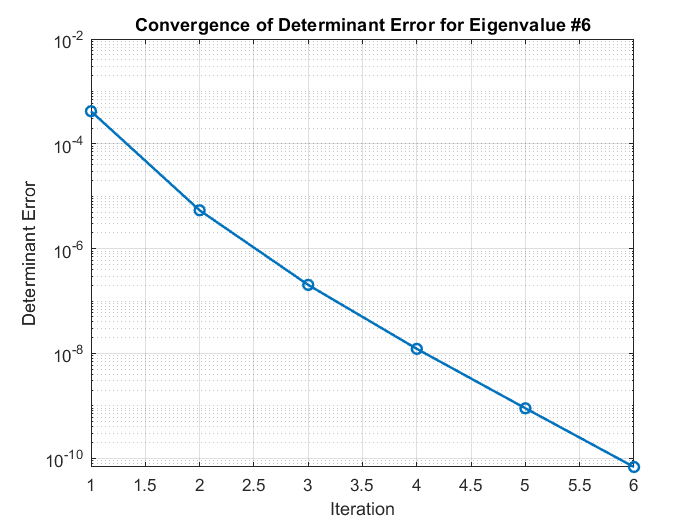
\includegraphics[width=\linewidth]{Figures/eigen_6.png}
%         \caption{Error Analysis 6}
%     \end{subfigure}
%     \hfill
%     \begin{subfigure}{0.3\linewidth}
%         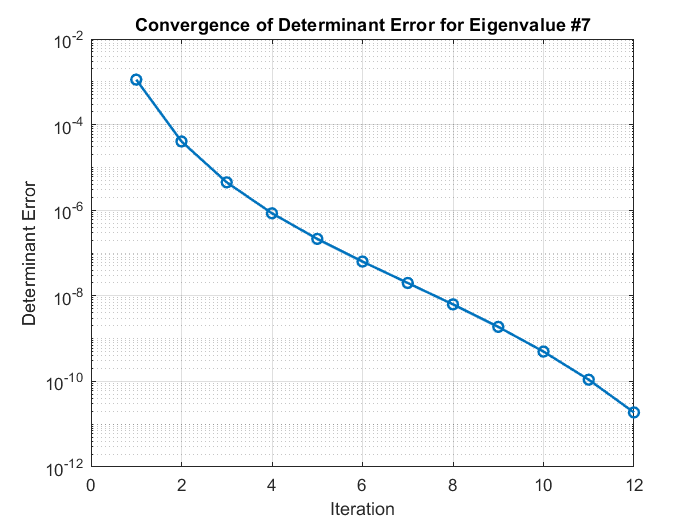
\includegraphics[width=\linewidth]{Figures/eigen_7..png}
%         \caption{Error Analysis 7}
%     \end{subfigure} 
%     \caption{Error analysis of the determinant for eigenvalue 1}
%     \label{graph-eigenvalue-01}
% \end{figure}

\end{example}


\newpage
\bigskip
\section{Applications of eigenvalues}
With the help of eigenvalues and eigenvectors, we can diagonalize a matrix and find its logarithm.

\begin{example}
Let
\[
A = \begin{bmatrix} 1 & 1 & 0 \\ 0 & 2 & 2 \\ 0 & 0 & 3 \end{bmatrix}.
\]

To find eigenvalues of $A$, firslty solve \(\operatorname{det}(A - \lambda I) = 0\) for \(\lambda\). This gives

\[
\operatorname{det}\begin{bmatrix} 1 - \lambda & 1 & 0 \\ 0 & 2 - \lambda & 2 \\ 0 & 0 & 3 - \lambda \end{bmatrix} = 0.
\]

The three eigenvalues of $A$ are \(\lambda_1 = 1\), \(\lambda_2 = 2\), and \(\lambda_3 = 3\).

We now calculate the eigenvectors associated to the eigenvalues \(\lambda_1 = 1\), \(\lambda_2 = 2\), and \(\lambda_3 = 3\).

For \(\lambda_1 = 1\), we have
\[
(A - I)\mathbf{v}_1 = \begin{bmatrix} 0 & 1 & 0 \\ 0 & 1 & 2 \\ 0 & 0 & 2 \end{bmatrix} \mathbf{v}_1 = \mathbf{0}.
\]

This gives 
\[
\mathbf{v}_1 = \begin{bmatrix} 1 \\ 0 \\ 0 \end{bmatrix}.
\]

Similarly, for \(\lambda_2 = 2\) and \(\lambda_3 = 3\), we have \(\mathbf{v}_2\) and \(\mathbf{v}_3\) as follows:
\[
\mathbf{v}_2 = \begin{bmatrix} 1 \\ 1 \\ 0 \end{bmatrix} \text{ and }
\mathbf{v}_3 = \begin{bmatrix} 1 \\ 2 \\ 1 \end{bmatrix}
\]

 Now we construct the matrices \(P\) and \(D\) as follows:
\[
P = [\mathbf{v}_1, \mathbf{v}_2, \mathbf{v}_3] = \begin{bmatrix} 1 & 1 & 1 \\ 0 & 1 & 2 \\ 0 & 0 & 1 \end{bmatrix}
\]
 
\[
D = \text{diag}(\lambda_1, \lambda_2, \lambda_3) = \begin{bmatrix} 1 & 0 & 0 \\ 0 & 2 & 0 \\ 0 & 0 & 3 \end{bmatrix}
\]

Now we calculate \(P^{-1}\) as follows:
\[
P^{-1} = \begin{bmatrix} 1 & -1 & 1 \\ 0 & 1 & -2 \\ 0 & 0 & 1 \end{bmatrix}
\]

Finally, we have the diagonal matrix $A = P D P^{-1}$ as follows:
\[
P D P^{-1} = \begin{bmatrix} 1 & 1 & 1 \\ 0 & 1 & 2 \\ 0 & 0 & 1  \end{bmatrix} \begin{bmatrix} 1 & 0 & 0 \\ 0 & 2 & 0 \\ 0 & 0 & 3 \end{bmatrix} \begin{bmatrix} 1 & -1 & 1 \\ 0 & 1 & -2 \\ 0 & 0 & 1  \end{bmatrix}
\]

Then we find $\log A$ as follows:
\[
\log A =  \begin{bmatrix} 1 & 1 & 1 \\ 0 & 1 & 2 \\ 0 & 0 & 1  \end{bmatrix} \begin{bmatrix} \log1 & 0 & 0 \\ 0 & \log2 & 0 \\ 0 & 0 & \log3 \end{bmatrix} \begin{bmatrix} 1 & -1 & 1 \\ 0 & 1 & -2 \\ 0 & 0 & 1  \end{bmatrix}
\]

\[
 =  \begin{bmatrix} 1 & 1 & 1 \\ 0 & 1 & 2 \\ 0 & 0 & 1  \end{bmatrix} \begin{bmatrix} 0 & 0 & 0 \\ 0 & \log2 & -2\log2 \\ 0 & 0 & \log3 \end{bmatrix}
\]

\[
 =  \begin{bmatrix}
   0 & \log2 & -2\log2+\log3 \\
   0 & \log2 & -2\log2+2\log3\\
   0 & 0 & \log3
\end{bmatrix}
.\]
% Now, $\operatorname{tr}(\log A) =  \log(2) + \log(3)$.
\end{example}